The advent of the internet brought forth the ability to share information with others in unprecedented time, and advancements in technology, like external storage, have revolutionized our access to knowledge. This nexus of limitless storage and real time capabilities has created a wealth of non-traditional forms of data that are decentralized, social, and crowd sourced. This presents a new challenge of how to store, quantify, and make sense of these new data sources. The democratization of information has culminated today in a dynamic crowd sourced encyclopedia vaster than anything before (Wikipeida.org), and in the social realm, social media sites  Twitter and Facebook have created a wealth of social interaction data. Since sharing in these mediums, is not subject to any linguistic or grammatical framework, it reveals organic interactions and highlights topics which matter to individuals. On Twitter, in particular, more voices are being heard than ever before with more than 500 million people generating over 340 million messages per day [citation needed - pew state of the twitter study?]. This data has been leveraged in the past to crush hard problems (FoldIt) [PNAS or science reference] and digitize all books (ReCaptcha) [citation needed] . 

Alongside these efforts, we seek to use text shared on Twitter to detect any collapse in language, or convergence on some particular topic, thereby computationally detecting the stories and topics that are being reported by individual users and shared across the network. Unlike traditionally news websites which fact check, write, rewrite, edit and then report, our news is reported by everyday people as soon as it is detected. We call this distributed news, and the aggregate tool the 'storyfinder.' The storyfinder uses two simple metrics elucidate the most surprising and emotional content during a fifteen minute window. Work in real time news extraction has been done before, but using machine learning techniques. We instead use alternative methods of conditional entropy and and ambient valence.  

We structure our paper as follows. In the Methods section, we describe a unique way to partition texts, define conditional entropy and ambient valence, and describe how the shifting process works. In our Results we apply the storyfinder to one week of Twitter data surrounding the 2013 Boston Marathon, and find that we pick up many key elements surrounding the bombings.\\




\textbf{Partitioning Text:}\\

Before any pattern analysis can occur, we need method to transform a large text, or in our case a large volume of tweets, into meaningful units of information. To do this we rely on a method developed by Williams et al.[citation needed]. First we create a probability distribution of all possible phrases in a text based on frequency of appearance in that text. We then go back and partition the same text using that probability distribution to find the optimal partition of phrases. It is important to note that the probability distribution represents the same text, such that all necessary phrases are included. Furthermore the partitions are completely disjoint and span the entire text. 

Are equations/ diagrams needed here?!  \\

\textbf{Computing Entropy of Phrases}\\

Once we have a partition of meaningful units, we can look at the context in which these units appear. We focus on the entropy of a phrase, which is computed within its local context (or clauses) using Shannon's entropy. A plunge in entropy indicates a collapse of language around central topics, indicating a possible story. 

For a phrase $p$, let $N_p$ be the count of $p$, let $\{ c_p \}$ be all of the neighborhoods of $p$, let $N_{c_p}$ be the count of neighborhood $c_p$ and then we define the entropy $E_p$ as
\[ E_p = -\sum _{c_p} N_{c_p} \log _2 \left ( N_p / N_{c_p} \right ) .\]
It is then necessary to normalize this over the sum of the neighborhoods so that we are getting at the probability of each neighborhood, so we set
\[ E_p = E_p / \sum _{c_p} N_{c_p} .\]

For a phrase, the value of entropy is limited by the frequency of appearance of the phrase.  Furthermore, since this measure of entropy is conditioned on a reference text, the entropy of a particular phrase is further limited the by length of the reference text. In our case, we compare the current fifteen minutes of tweets to the past fifteen minutes of tweets.  By only using the fifteen minutes prior, we can pick up a diurnal cycle as well as find the shapes of stories. \\

\textbf{Computing Ambient Valence of Phrases}\\

Another metric we use to find stories is ambient valence. This measure is intended to be capture a more psychological aspect of stories: happiness. Some of the biggest stories we share, are either very sad or very happy, and we hope to capture the changes in happiness using a method developed by Dodds et al [citation needed]. The LabMT dataset contains 10222 words with happiness scores on a 1 to 9 scale, averaged over 50 independent ratings through Mechanical Turk.To extend the valence scores on words into scores on phrases, we compute the ambient valence of a phrase $p$ be averaging the scores of all the words surrounding this phrase for which we have scores.
% As was shown by Dodds et. al., this instrument is tunable to the removable of neutral words.
% We test this tunability on ambient phrase scoring by considering the correlation of the happiness timeseries on Twitter.
The correlation between valence and ambient valence of words in the LabMT set in Figure \ref{fig:ambwordcor} provides some evidence for the validity of this scoring, showing a positive trend with correlation $\rho = .51$.\\



\begin{figure}[tpb!]
\centering
  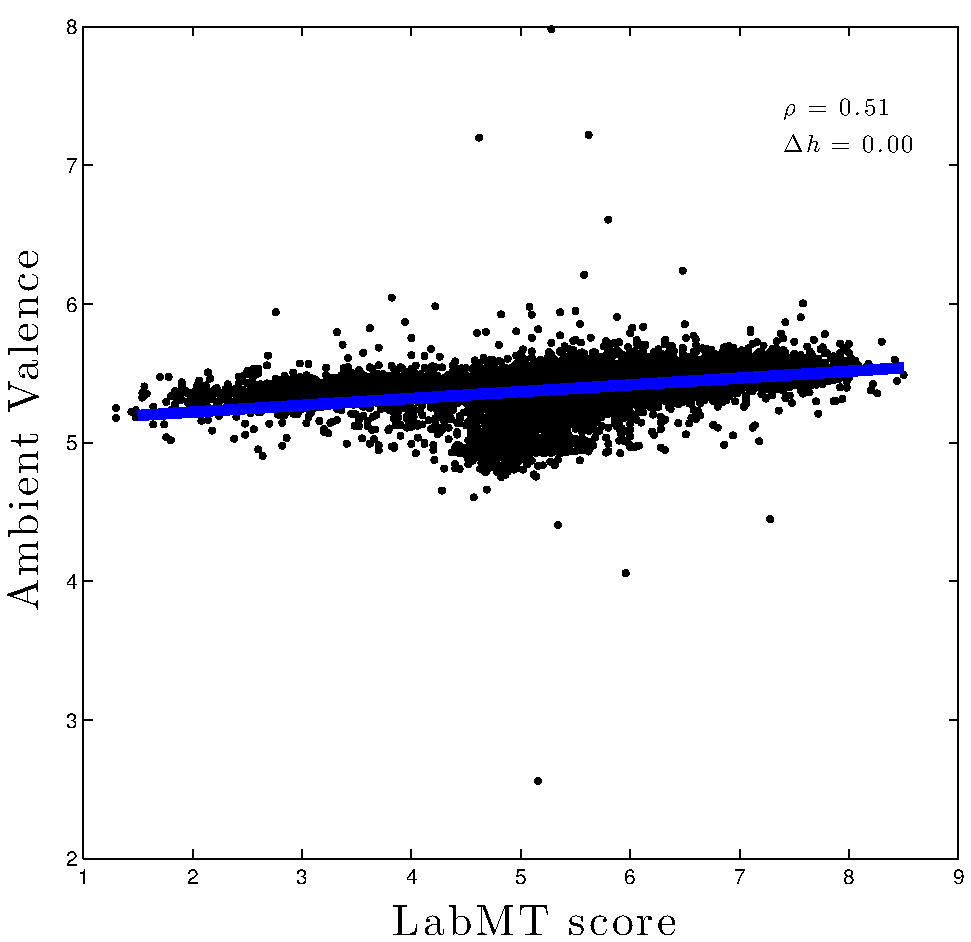
\includegraphics[width=.45\textwidth]{../MTambVal_000_plot_noname.pdf}
  \caption{
    The valence and ambient valence of words in the LabMT set.
  }
  \label{fig:ambwordcor}
\end{figure}


We next will perform a validation of the choice for $\Delta h = 0$ for this application via a timeseries correlation, in addition to the LabMT word correlations presented as in Figure \ref{fig:ambwordcor}, which we include in the supplementary for more choices of $\Delta h$.\\


\textbf{Shifting Phrases Measures Against a Reference}\\

When a significant change in the entropy or valence of language occurs, we desire to find the phrases most responsible for this change to indicate the event.
The difficulty here is that specific phrases can contribute to changes in entropy and valence in many ways, since the entropy and valence of that phrase can change.
For valence, this shift is written as
\begin{equation} h_\text{avg} ^\text{(comp)} - h_\text{avg} ^{(ref)} \label{eq:valenceshift} \end{equation}
where $h_\text{avg} ^\text{(comp)}$ is the valence of the text in question and $h_\text{avg} ^\text{(ref)}$ is the valence of the reference text.

\begin{figure}[tpb!]
\centering
  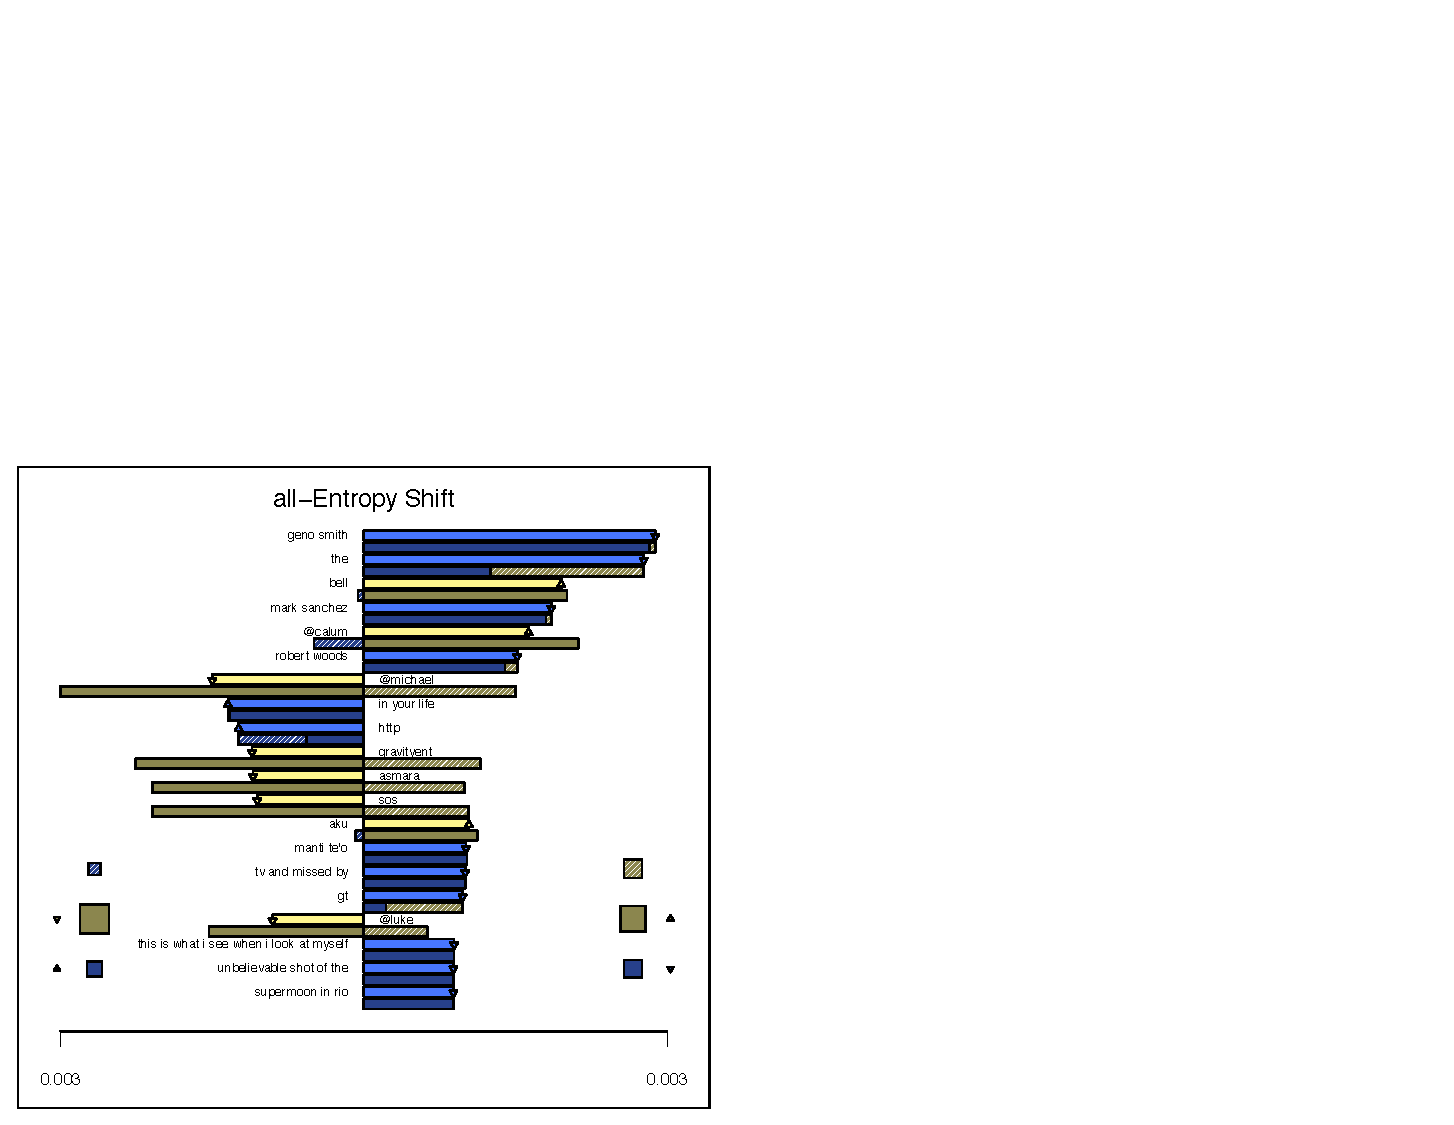
\includegraphics[width=.45\textwidth]{../example_valence_shift.pdf}
  \caption{
    An example entropy shift shows each of the ways that a phrase can contribute to a changing entropy.
  }
  \label{fig:exshift}
\end{figure}

There are many ways to break down equation \ref{eg:valenceshift}, and what we find to give the most insightful breakdown of contributions is analogous to the 2-dimensional derivative.
This is writing Eq \ref{eq:valenceshift} as, for each word $w$ with happiness $h_w$ and probability of appearance $P(w)$,

\begin{figure}[tpb!]
\centering
  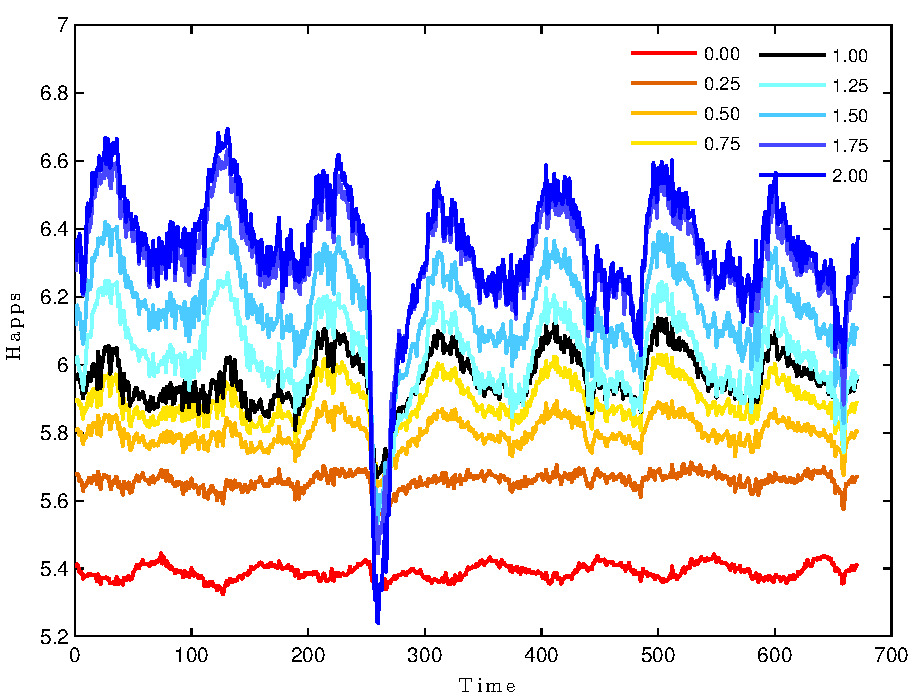
\includegraphics[width=.45\textwidth]{../timeseries_noname.pdf}
  \caption{
    Valence timeseries on the dates surrounding the Boston Marathon.
    Ambient valence is computed every 15 minutes.
    Different values of $\Delta h$ are tested, and we choose $\Delta h = 1$ for ambient valence calculation, as in \cite{hedo-2011}.
  }
  \label{fig:timeseries}
\end{figure}


\begin{equation} \sum _w \left ( h_w ^\text{(comp)} - h_w ^\text{(ref)} \right ) \left ( P(w) ^\text{(comp)} - P(w) ^\text{(ref)} \right ) . \end{equation}

This is represented by Figure \ref{fig:exshift} for the top bar for each word, as the total contribution to the change in valence by that word.
The two bars below represent the two ways in which a word shifted the signal: from a change in valence in the text, and from a change in frequency.
The dashed bars represent the change in frequency, and the solid bars represent the change in frequency.
Color indicated whether, relative to the comparison text, the phrase is above the average (whether it is happy).
We are able to show the two bars by rewriting the sum above into two terms in the following equation:
\begin{align*} & \sum _w h_w ^\text{(comp)} \left ( P(w) ^\text{(comp)} - P(w) ^\text{(ref)} \right )\\
& ~~~~~~~~~ + \sum _w\left ( h_w ^\text{(comp)} - h_w ^\text{(ref)} \right ) P(w) ^\text{(comp)} .\end{align*}

\begin{figure}[tpb!]
\centering
  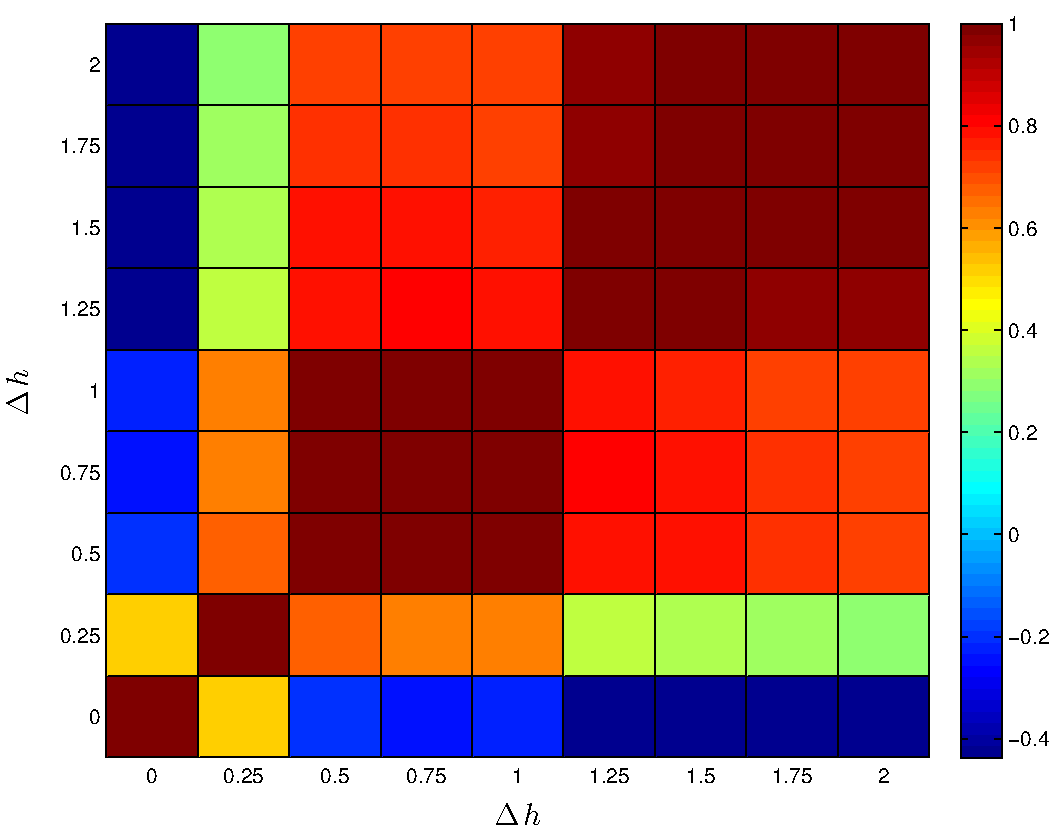
\includegraphics[width=.45\textwidth]{../correlationMatrix.pdf}
  \caption{
    Correlation of different valence timeseries using different values of $\Delta$ h.
  }
  \label{fig:corrMatrix}
\end{figure}

\textbf{Preliminary Results with Twitter Data}\\

Applying the above methodology to data from Twitter's Streaming API during the week of the Boston Marathon we hope to be able to see the events that took place through this lens.
An example timeseries in Figure \ref{fig:timeseries} for the six days ranging from April 18 through April 26 provides a picture of what we measure for entropy and valence over the week.
The entropy and valence shifts below correspond to shifting the most recent 15 minutes of Twitter data against the 15 minutes prior.
Choosing the window with which to bin tweets, and the reference text are important future considerations.
Our current setup is shifting the current 15 minutes against the previous day, and future experiments will attempt to optimally combine reference texts for the option of attempting to remove the daily cycles that do not represent large events.
Note the inaccuracies in the data of Figure \ref{fig:timeseries} in the caption, but notice that we do see two significant downward spikes in entropy on April 19. We'll zoom in on those.\\


\begin{figure*}
\centering
  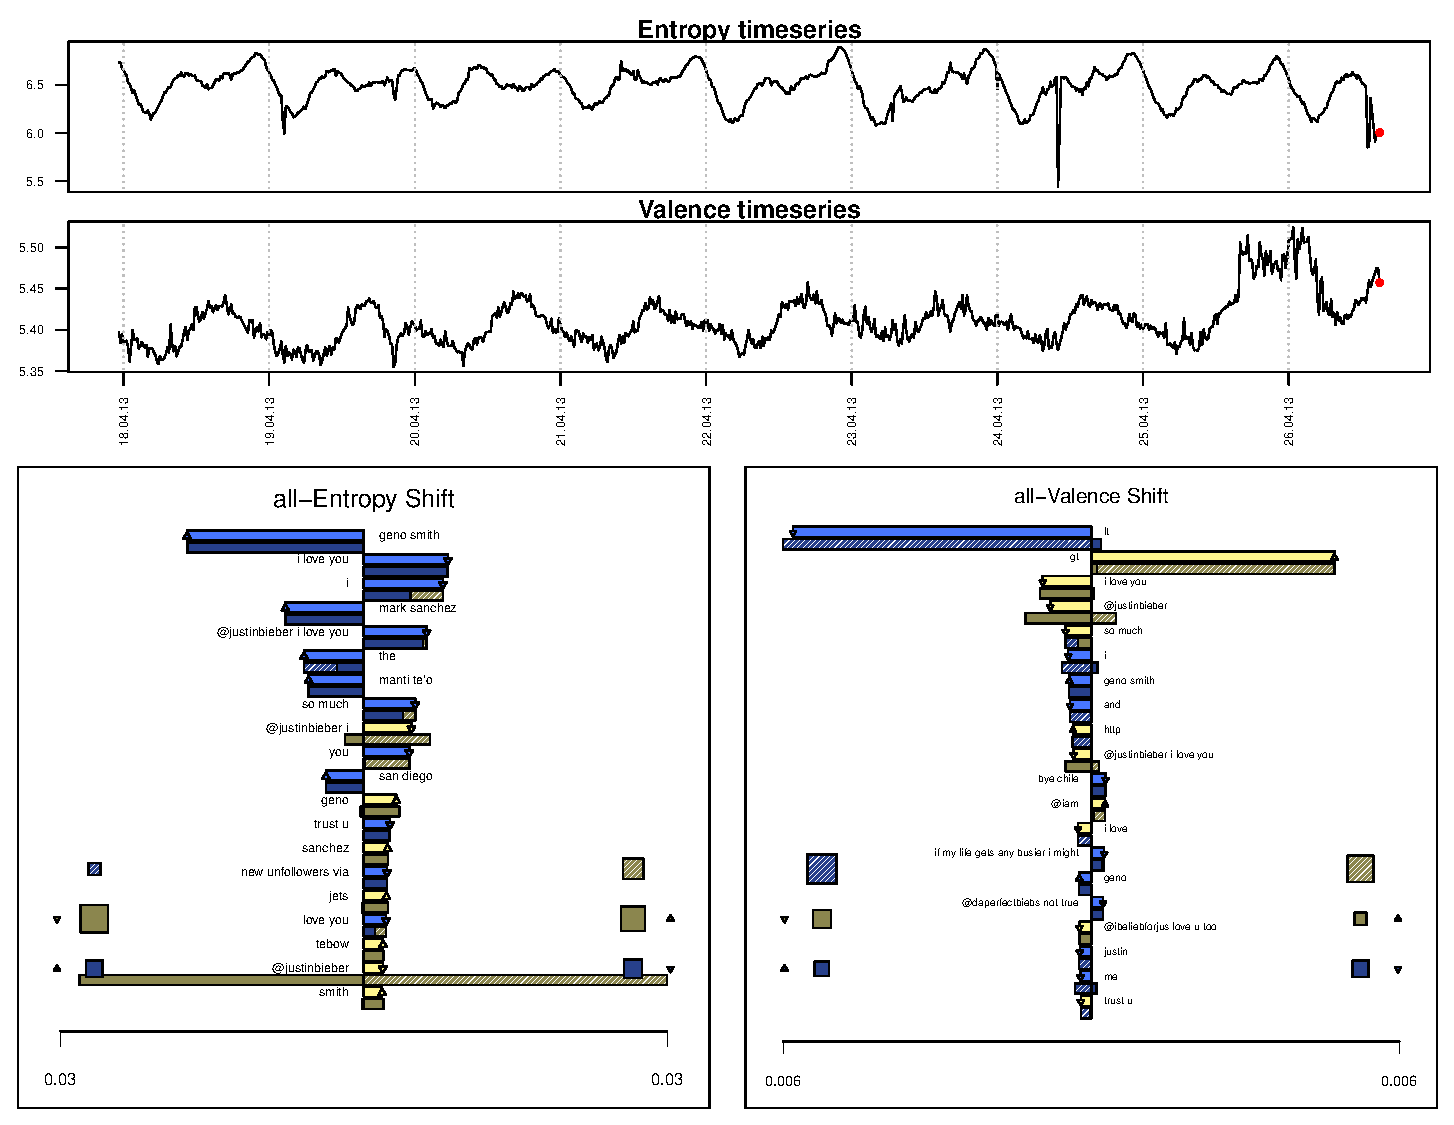
\includegraphics[width=\textwidth]{../example_timeseries2.pdf}
  \caption{
    April 18 through April 26 on Twitter, with shifts plotted for the most recent 15 minutes against the 15 minutes prior.
    Some of the variations are artifacts of this being a work in progress, and halting our current experiment for hedonometer.org (check it out!): namely the downward spike in the middle of April 25th, and the upward valence bubble near the end are not accurate.
  }
  \label{fig:timeseries}
\end{figure*}

\begin{figure*}
\centering
  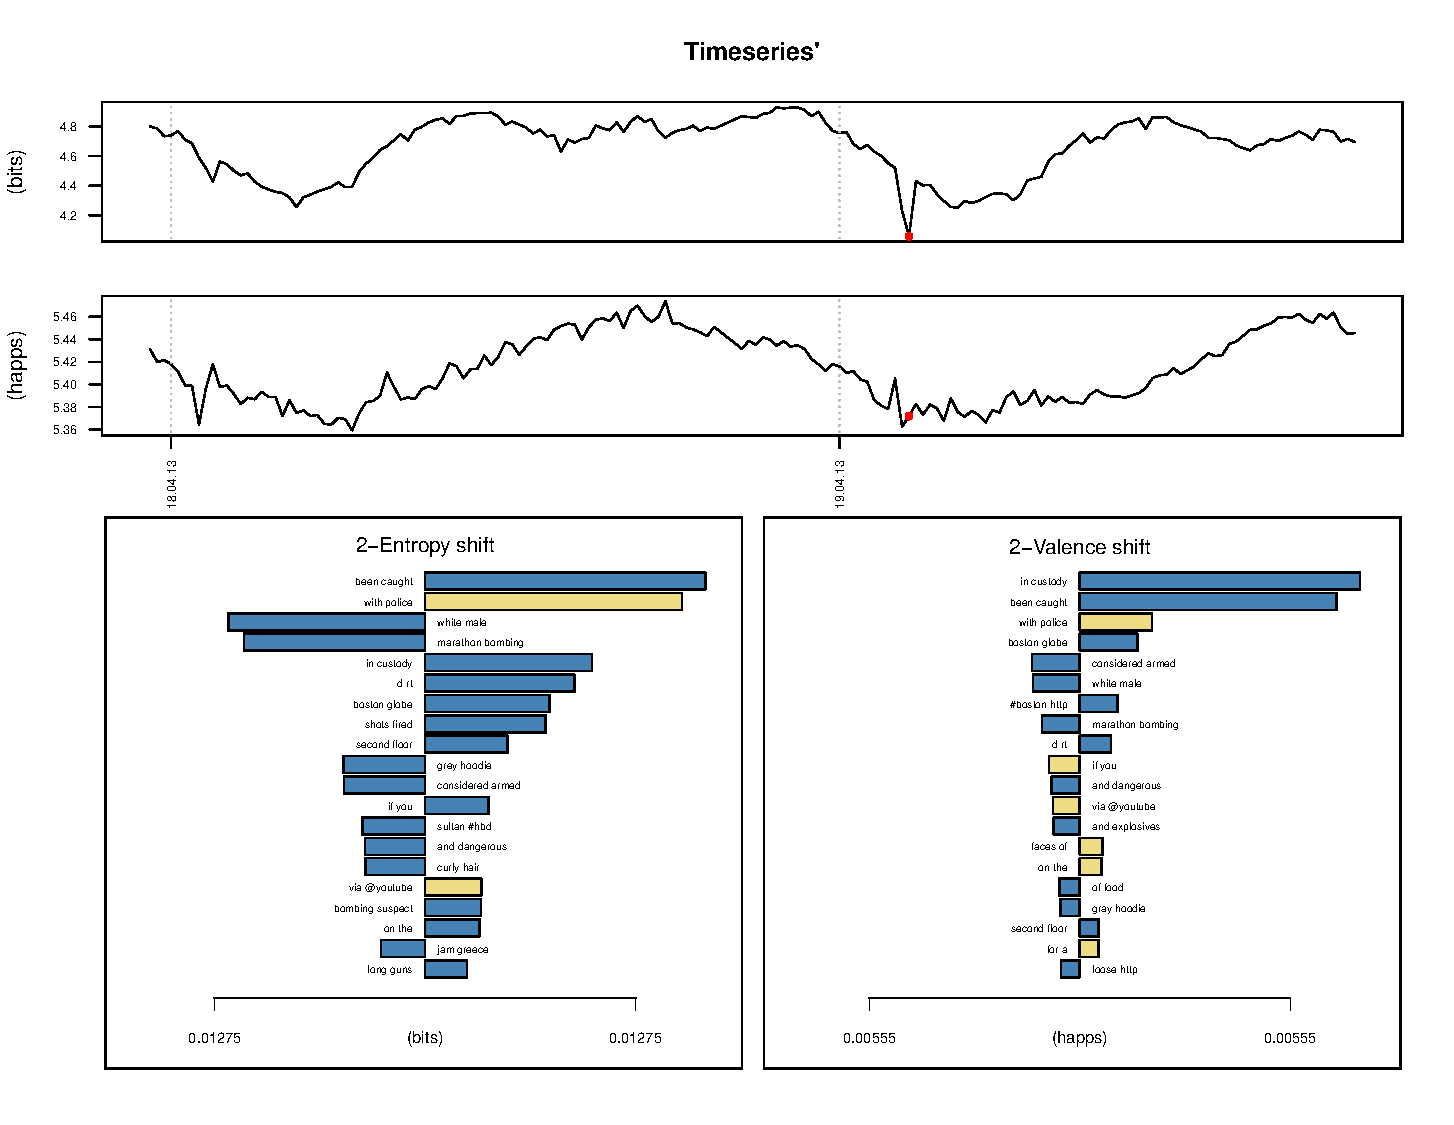
\includegraphics[width=\textwidth]{boston1.pdf}
  \caption{
  Looking at the length two shifts when we see the first downward spike on Apr 19.
  The words make the story clear, and we recognize that this is the time at which the first bomber was caught.
  }
  \label{fig:timeseries_boston1}
\end{figure*}

\begin{figure*}
\centering
  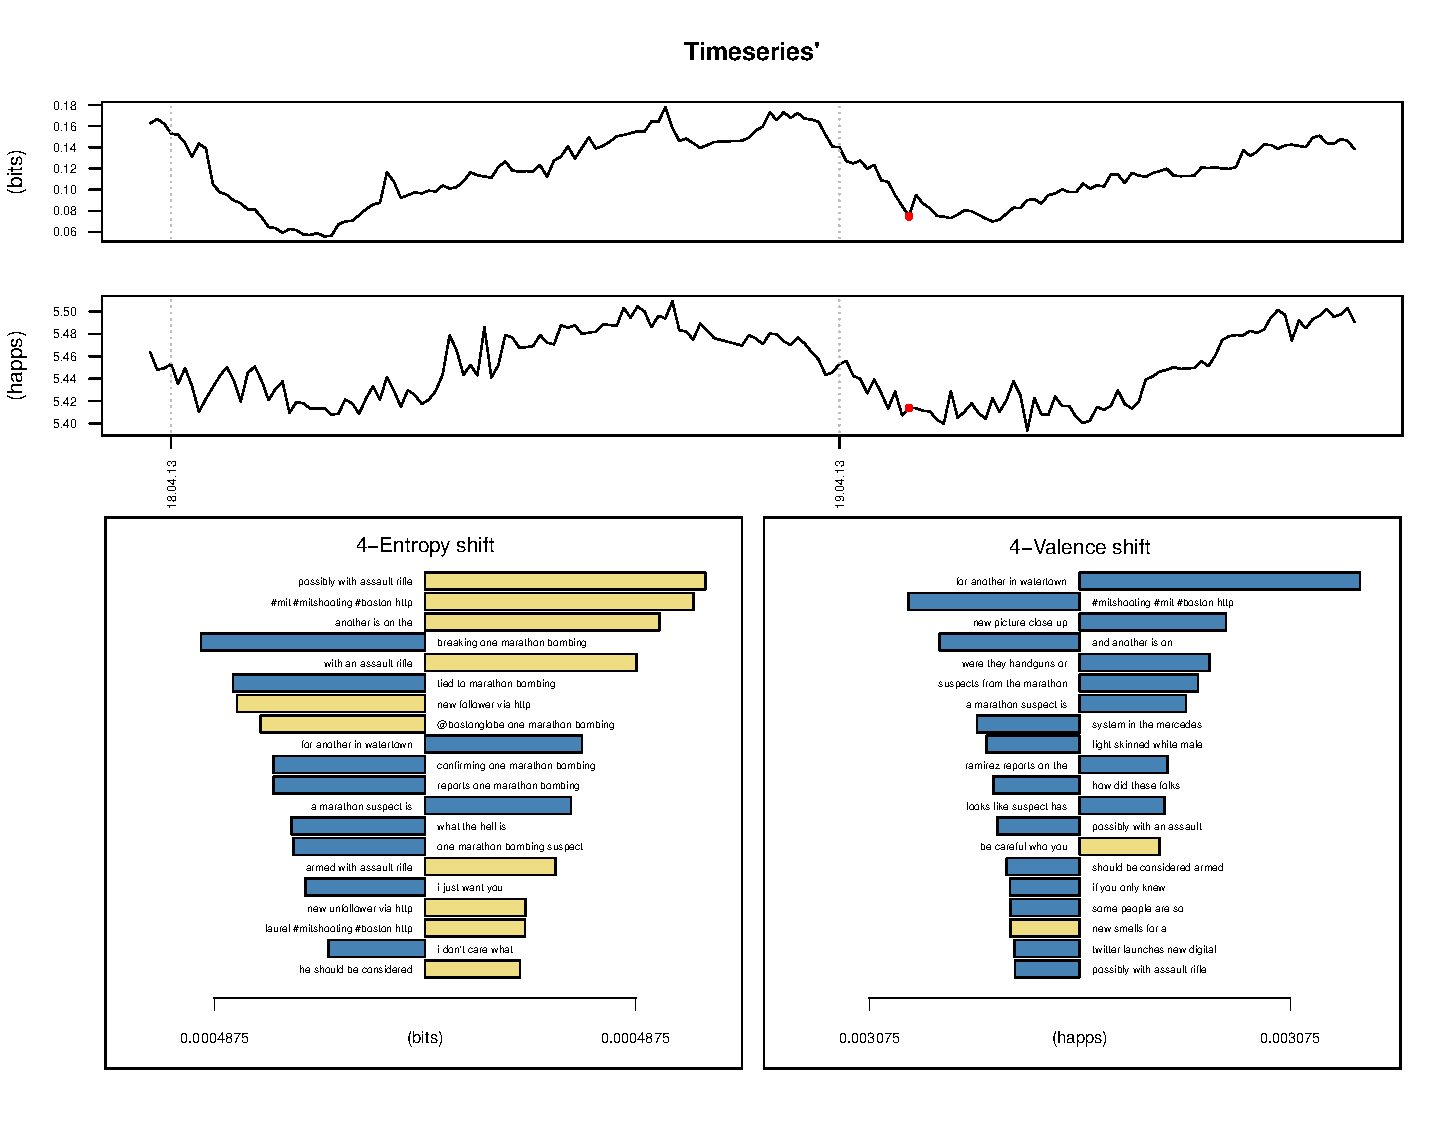
\includegraphics[width=\textwidth]{boston2.pdf}
  \caption{
  The same time as \ref{fig:timeseries_boston2}, looking at length 4 sequences.
  }
  \label{fig:timeseries_boston2}
\end{figure*}

\begin{figure*}
\centering
  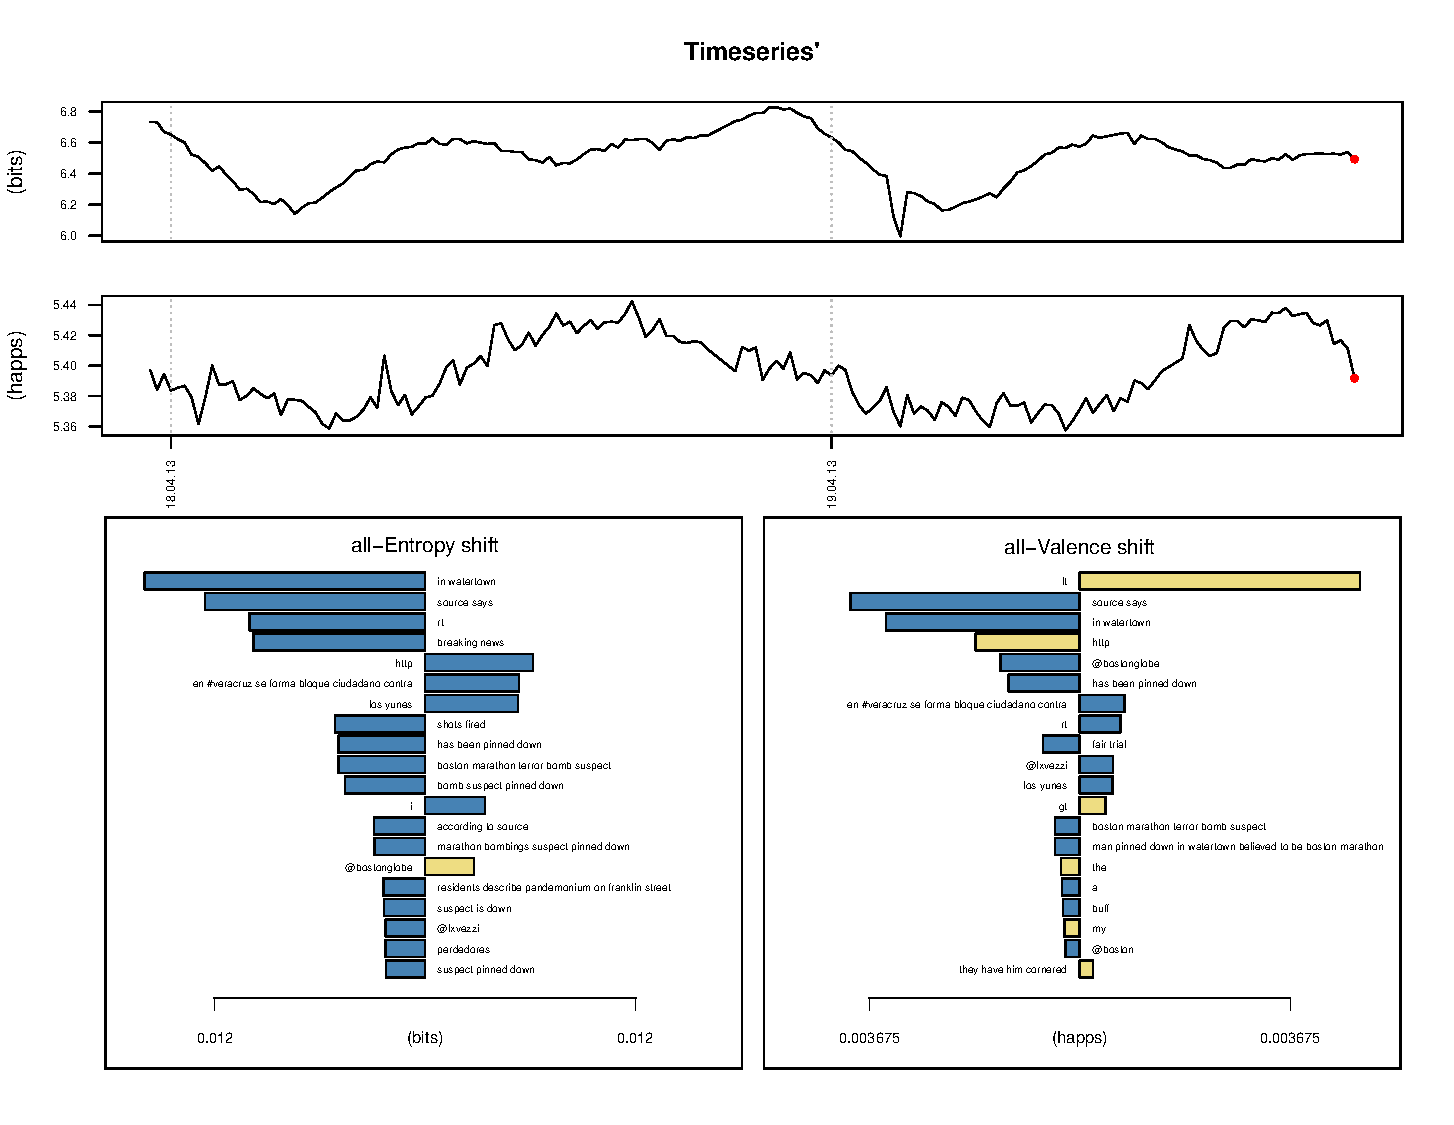
\includegraphics[width=\textwidth]{boston3.pdf}
  \caption{
  The all valence shift for the second dip in entropy, later on the 19th, about 10PM.
  The word shifts show us that this is when the final suspect is caught.
  }
  \label{fig:timeseries_boston3}
\end{figure*}

\begin{figure*}
\centering
  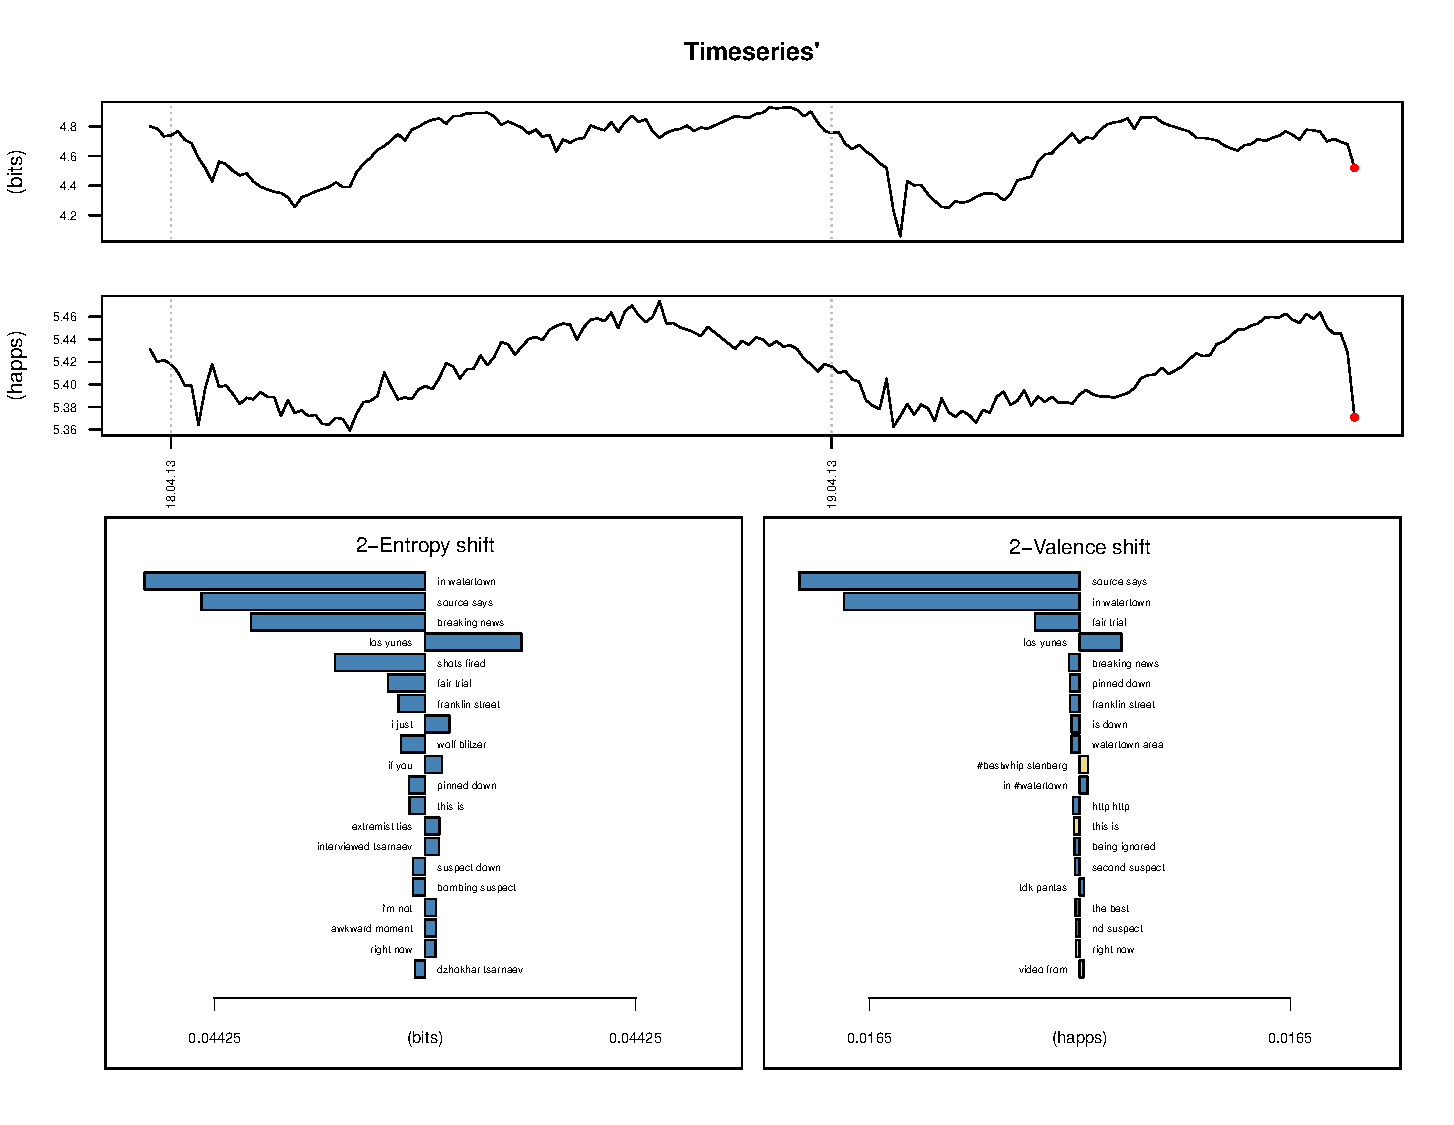
\includegraphics[width=\textwidth]{boston4.pdf}
  \caption{
  The same time as \ref{fig:timeseries_boston3}, looking at the 2-grams.
  The cool thing here is, we pick up ``franklin street'', the location of the shootout, which was at the time classified information.
  }
  \label{fig:timeseries_boston4}
\end{figure*}



\textbf{Conclusion:}\\

We show that our story finder is successful in distilling information in a timely manner, when applied to the case study of the Boston Marathon. We find the initial bombing, the names of the suspects, the MIT shooting, even precise locations such as Franklin St. We hope to use this tool as a forecaster of important news, but also as an instrument to study the characteristics of stories. 



\end{document}
